\documentclass[HardwareDesign/HardwareDesign_main.tex]{subfiles}
\begin{document}
\section{Cup Holder}\label{sec:cupholder_hw_design}
I dette afsnit beskreves design og implementeting af Cup Holder.

\subsection{Design}
Cup Holder består af de to delkomponenter Cup Light og Cup Sensor. Disse delkomponenter er allerede designet og det eneste der skal gøres er at sætte disse to sammen. Der skal dog også være nogle stik så Cup Holder kan forbindes til Power Supply og Cup Holder Controller.
Designet kan ses på figur \ref{fig:CupHolderDesign}. Designet er lavet i multisim, og de to diagrammer for Cup Light og Cup Sensor importeres som en 'Hierarchical block'. Dette er de to blokke HB2 og HB1. Derudover er der de to førnævnte stik. J1 er stikker til Power Supply og J2 er stikket der bruges til forbindelsen til Cup Holder Controller. 

\begin{figure}[H]
    \centering
    \makebox[\textwidth][c]{%
        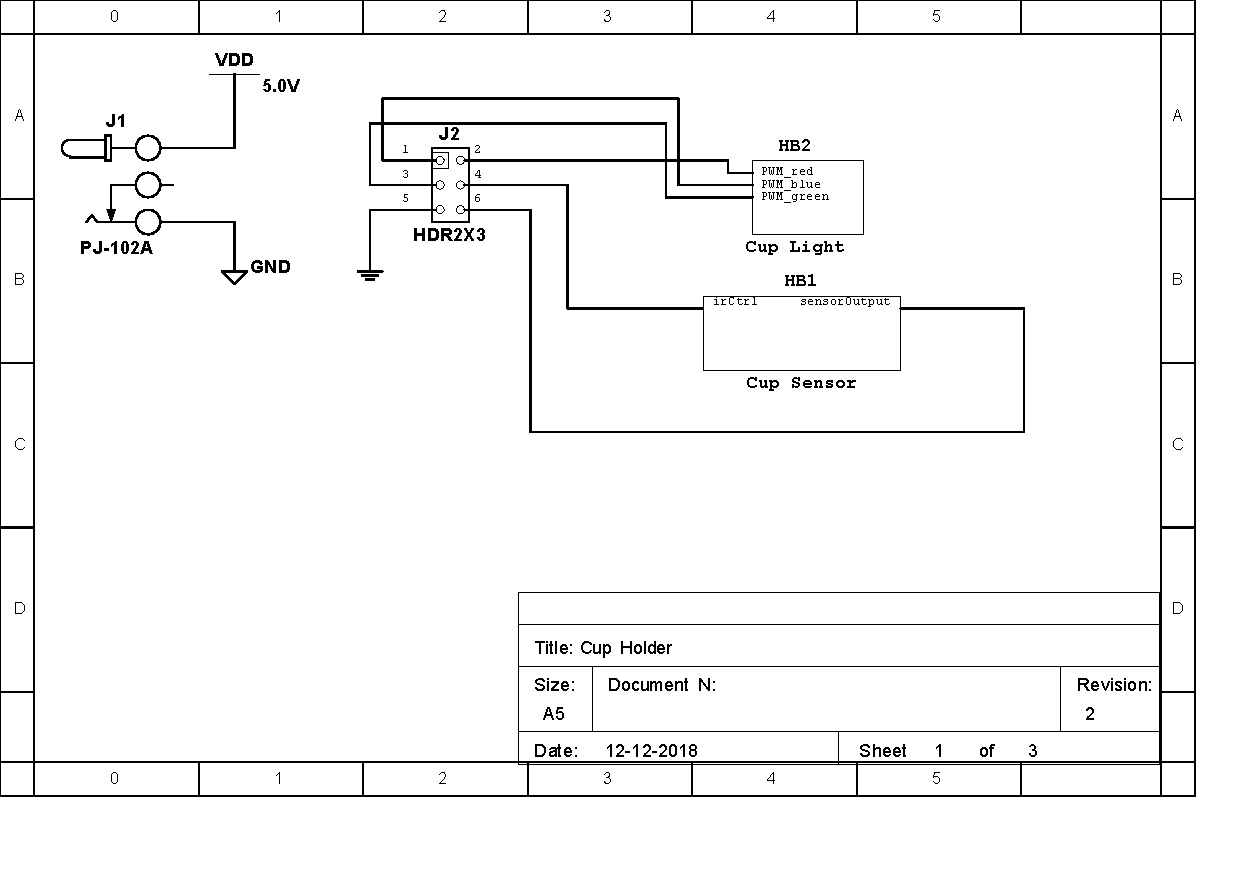
\includegraphics[width=1\columnwidth,trim={0.24in 2.8in 1.2in 0.24in},clip, page=1]{HardwareDesign/CupHolder/graphics/CupHolder.pdf}
    }
    \caption{Design af Cup Holder}
    \label{fig:CupHolderDesign}
\end{figure}

Cup Holder implementeres som en printplade. Denne printplade skal derfor også designes. Det vigtigste der er fokuseret på medhensyn til denne printplade er de fysiske dimensioner, heribland placering af komponenterne, og der fokuseres også på støj. Der står i krav specifikationen at RGB LED'erne fra Cup Light skal være i en ring rund med en diameter på $65\si{mm} \pm 1\si{mm}$, se ikke funktionelle krav K\ref{kravspec:req:light-D-center} i kravspecifikation. Derudover skal vinklen mellem hver LED være $70^{\circ} \pm 2^{\circ}$., se ikke funktionelle krav K\ref{kravspec:req:light-led-angle}. Det vil sige at de skal være jævnt fordelt. RGB LED'er er derfor placeret som beskrevet i kravene. Som en del af designet af Cup Sensor blev det bestemt at den infrarøde LED skal være i centrum af Cup Holder og at afstanden mellem IR LED'en og en fotodiode skal være 4 modulafstande (10.16mm). De fire fotodioder skal derudover være placeret på en cirkel med en radius på 10.16mm og de skal være jævnt fordelt på cirklen (90 grader mellem dem). Det sidste krav der er til placering af komponenterne er at de to stik skal være i kanten af printpladen. Derudover er det også valgt at printpladen skal være rund, da de fleste af komponenterne er placeret i en cirkel, men også da det gør det lettere at have flere Cup Holders ved siden af hinanden.

Der blev i projektet udviklet to printplader, som er stort set identiske, udover små ting som skulle tilpasses til produktionen af dem. Det første version var der fx. ikke gennemplatering. Der blev lavet to versioner, da der i første omgang kun blev lavet en (til test), og derefter blev der lavet 12 styk, som af økonomiske oversager skulle laves et andet sted og derfor blev printpladen modificeret en smule. Den endelige printplade kan ses på figur \ref{fig:CupHolderPrintpladeDesign}.

\begin{figure}[H]
\centering
\makebox[\textwidth][c]{%
\begin{subfigure}{.55\textwidth}
  \centering
        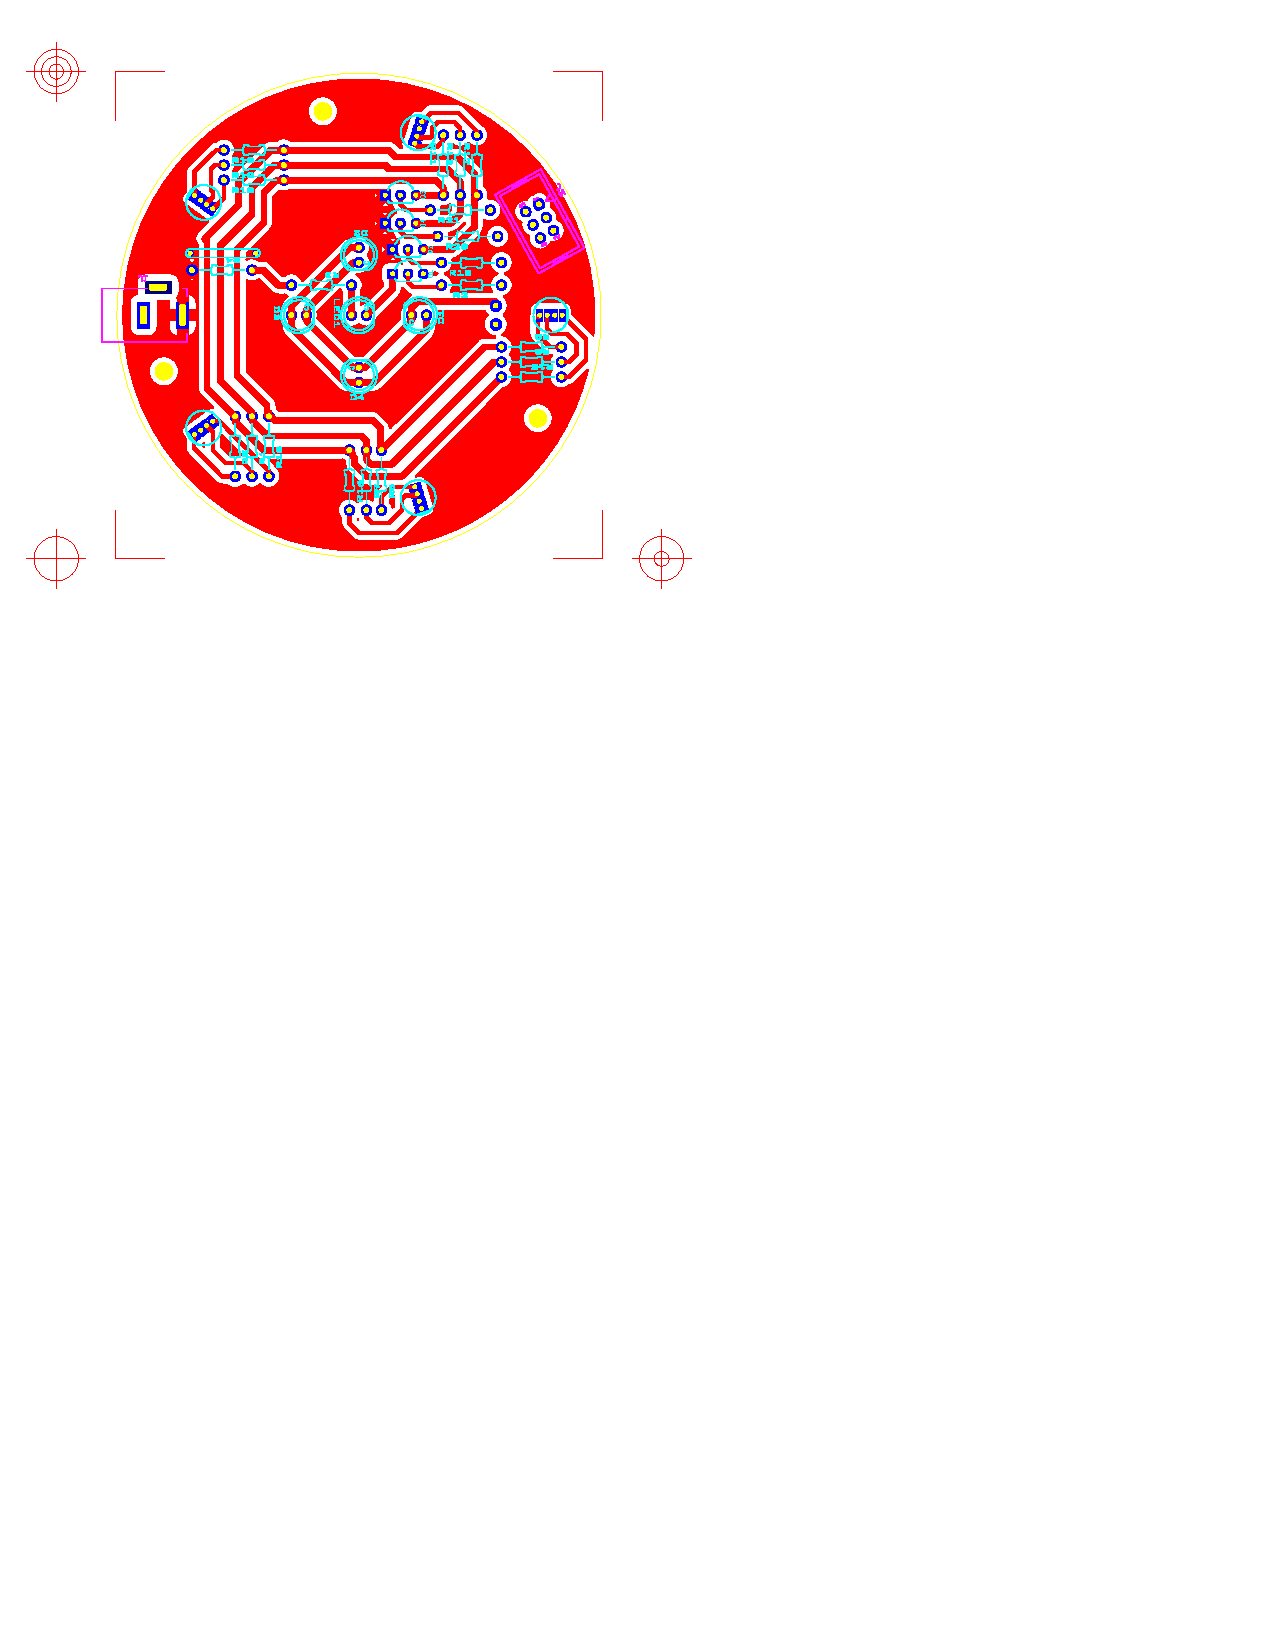
\includegraphics[width=1\linewidth,trim={0.6in 7.28in 4.5in 0.5in},clip, page=1]{HardwareDesign/CupHolder/graphics/bund.pdf}
\end{subfigure}%
\begin{subfigure}{.55\textwidth}
  \centering
    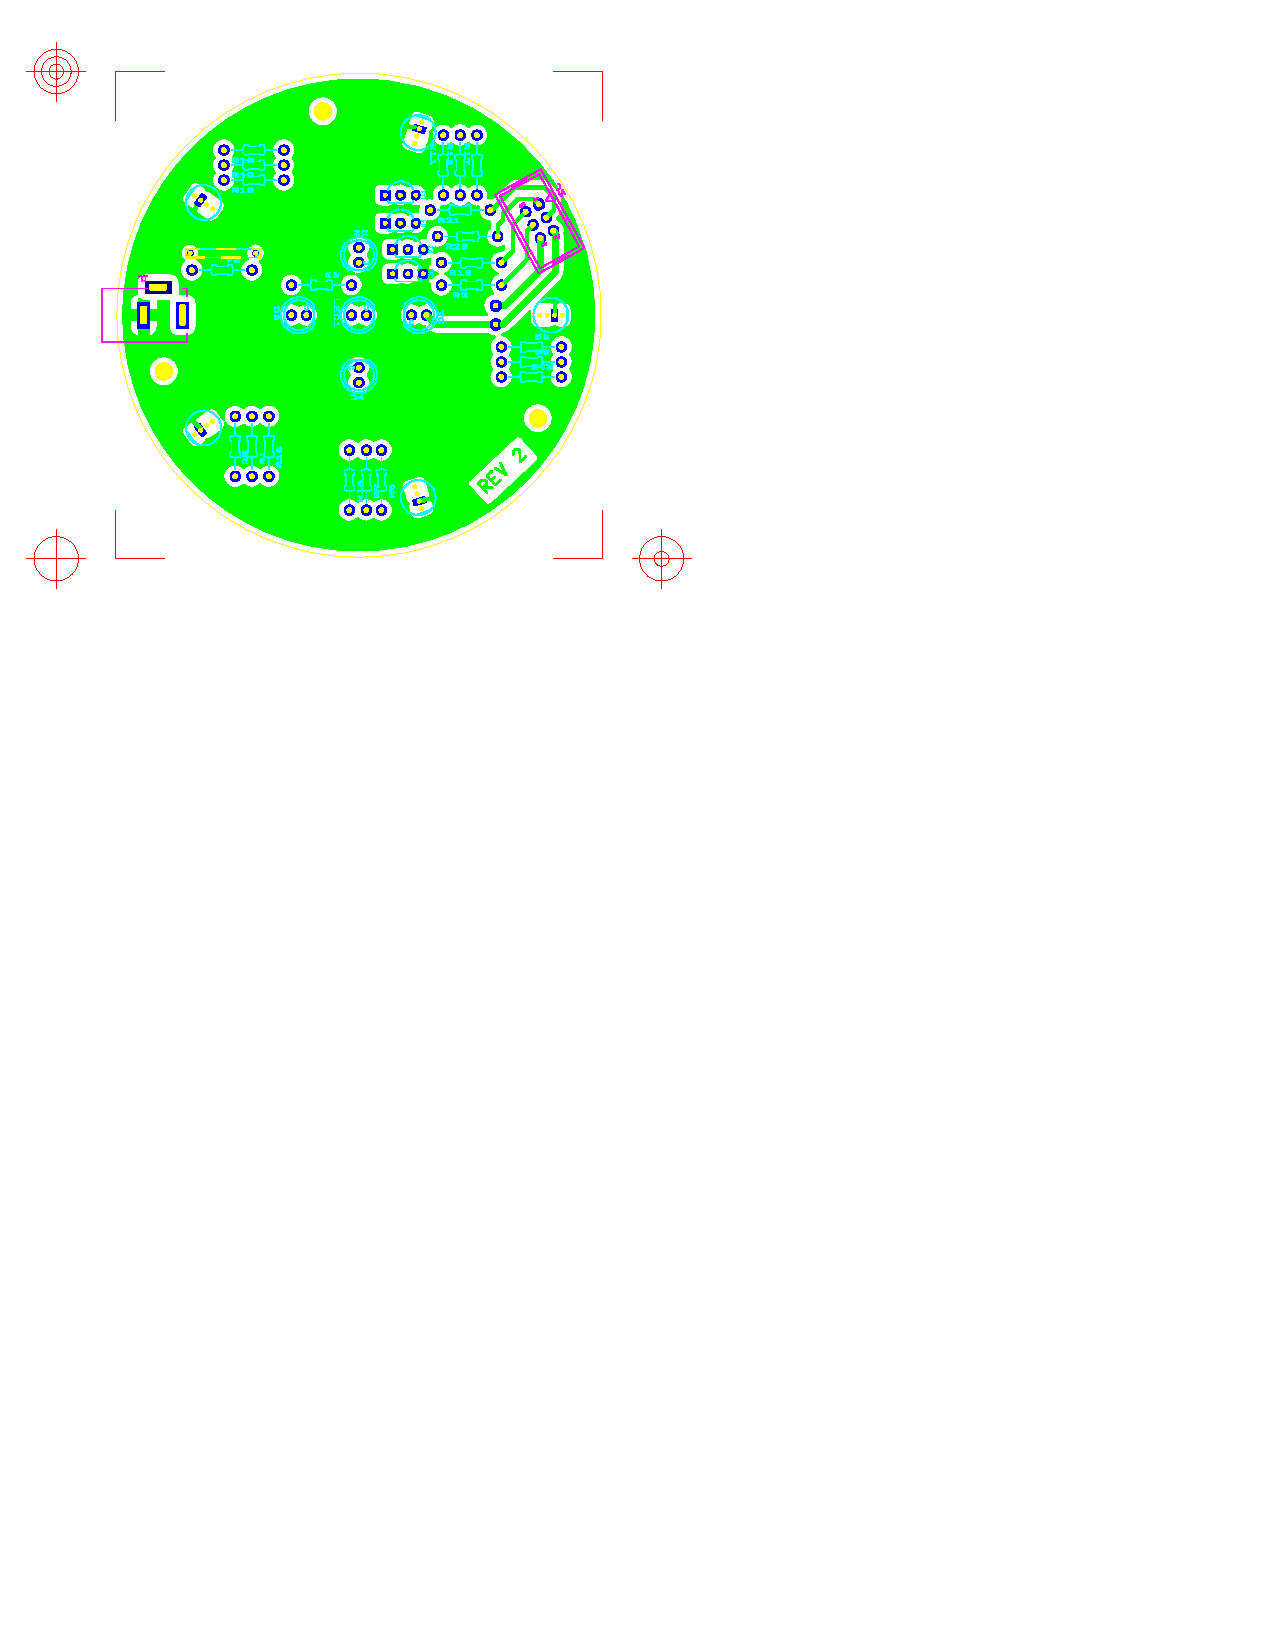
\includegraphics[width=1\linewidth,trim={0.6in 7.28in 4.5in 0.5in},clip, page=1]{HardwareDesign/CupHolder/graphics/top.pdf}
\end{subfigure}
}
\caption{Design af printplade. På venstre figur er det røde areal kobberet på undersiden af printpladen og på højre figur er det grønne areal kobberet på oversiden. Den cyane farve er silkscreen på toppen, som viser hvilke komponenter der er på oversiden. Den lilla farve er silkscreen på bunden og indikerer komponenter der sidder på bunden}
\label{fig:CupHolderPrintpladeDesign}
\end{figure}


\subsubsection{Støj}
Som det (lidt utydeligt) ses på \ref{fig:CupHolderPrintpladeDesign} er komponenterne placeret som tidligere beskrevet. Den næste vigtige del af design af printpladen er støjovervejelser. Der overvejes kun støj mellem de to delkomponenter Cup Light og Cup Sensor. Støj fra eksterne kilder tages derfor ikke i betragtning. Derudover fokuseres der kun på den støj som Cup Light forårsager på Cup Sensor og ikke den anden vej, da Cup Sensor er den som er mest sensitiv over for støj. De forskellige støjkoblinger der overvejes er induktiv kobling, kapacitiv kobling og fælles strømvej.

\paragraph{Fælles strømvej} For at minimere den fælles stømvej er det valgt at seperere de to komponenters stel. De vil dog ende med at have fælles stel på Cup Holder Controller, men jo mindre fælles stel de har jo bedre. Dette gøres ved at ben 5 på J2 er stel for fotodioen på Cup Sensor. De andre dele for stel fra J1. 

\paragraph{Kapacitiv kobling} Da der til styring af RGB LED'erne benyttes PWM signaler, som er en ændringer i spænding, kan disse signaler give anledning til kapacitiv støj. For at minimere den kapacitive støj er det forsøgt at have signalerne til RGB LED'erne så langt væk fra signalerne til fotodioderne. Det ses på figur \ref{fig:CupHolderPrintpladeDesign} at der er forsøgt at have de tre parallele ydre baner (banerne som forbindes til de 5 RGB LED'er) så langt væk fra de sensitive parallele baner i centrum (banerne der forbinder de fire fotodioder. Det har dog ikke altid været muligt. Fx er signalerne på transitorne meget relativt tæt på de sensitive baner.

Til at regne på støjen, findes det sted hvor afstanden mellem de støjende signaler og de sensitve signaler er kortest, og herefter antages det at der er denne afstand helle vejen rundt i en cirkel. Denne afstand bestemmes til ca. 6mm. Den støjende banen er her 18mm fra centrum. Det antages at de er parallele og i en længde er $l = 2\pi\cdot18\si{mm}$. Begge baner er 1mm tykke, forholdet mellm tykkelse $B=1\si{mm}$ og afstanden mellem dem $A=6\si{mm}$ er derfor $\frac{A}{B} = 6$. Derfor er kapaciteten mellem de to baner ca. $25\si{\frac{pF}{m}}$ og kapciteten er derfor $C=25\si{\frac{pF}{m}}\cdot2\pi\cdot18\si{mm} = 2.8 pF$. Hvis det antages at alt spændingen vil være over denne kapacitet vil strømmen igennem den være $i = C \frac{dv}{dt}$ Det blev i modultesten for Cup Light målt at stige tiden på spændingen over modstanden er 22ns. Hvis det antages at spændingen stiger lineært er gælder følgende: $\frac{dv}{dt} = \frac{5\si{V}}{22\si{ns}} = 230\si{\frac{MV}{s}}$
strømmen er derfor $i = 2.8pF \cdot 230\si{\frac{MV}{s}} = 644\si{\mu A}$. I værste tilfælde vil der være en støjspids på $644\si{\mu A}$, i lidt over 22ns. Selve amplituden af dette støj er høj. I realiteten vil støjen være mindre, fordi der ikke her den samme afstand hele vejen rundt. Derudover antages det også at der ikke er nogen nogen modstande i systemet, som fx. i forsyningsspændingen eller i transitorne som styre signalet. Det er forsøgt at minimere støjen, ved at der er et stelplan på stort set hele overfladen af printpladen, og et 5V plan på undersiden. På denne måde vil støjen kobles til stel/5V og ikke så meget sensoren.

\paragraph{Induktiv kobling} Da der løber en relativ stor strøm til RGB LED'er som ændre sig relativt hurtigt, vil en evt. induktiv kobling støje relativt meget. For at minimere den induktive kobling sørges der for at returbanerne er så tæt på signalbanerne som muligt. Dette er for magnetfeltet fra strømmen i den ene retning vil udligne magnetfeltet fra strømmen i den anden retning. På denne måde vil der være et minimalt magnetfelt som skal generere støj i Cup Sensor delen. For at returbanerne er så tætte på signalbanerne som muligt benyttes igen stelplanet. Her vil signalerne automatisk anbringe sig så der genereres mindst mulig støj.

\paragraph{Er støjen et problem?}
Begge støjsignaler vil opstå som spike idet det digitale signal skifter. Dette vil være spikes på lidt over 22ns. Dette tænkes ikke at det vil påvirke CupSensor signalet så meget, da i designet for Cup Sensor er implementeret et båndpasfilter i form at en ADC med indbygget mixer-funktionalitet og lavpasfilter. Båndpasfilteret har en centerfrekvens på 10kHz og en båndbredde på under 4kHz Frekvensindholdet for et så kort et spike, er meget høj og det bliver derfor dæmpet meget.

\subsection{Implementering}
Der blev først udviklet én printplade som blev produceret af ASE, denne version kan ses på figur \ref{fig:CupHolderRev1}. Denne version blev verificeret og der blev bestilt 12 printplader. Dette var ikke muligt at få produceret af ASE, derfor for blev den produceret i Kina (leverandør ikke oplyst af ASE), se figur \ref{fig:CupHolderRev2}. Her var det muligt at benytte gennemplatering, derfor blev der lavet en lidt anderledes version (REV 2). Begge versioner benytter afstandsstykker, som bruges til at printpladen kan stå på en flad overflade, og så der på toppen kan være en plastikplade. Det observeres at der på den REV 2 ikke er monteres 5 RGB LED'er. Detter var af økonomiske oversager det det vil koste lidt under 500kr for LED'erne og da lyset ikke har anden opgave end lir. Derfor loddes kun en på, det anses som værende tilfredsstillende kun at have en LED på REV 2 når der blev monteret 5 på den første version.

\begin{figure}[H]
\centering
\makebox[\textwidth][c]{%
\begin{subfigure}{.539\textwidth}
  \centering
        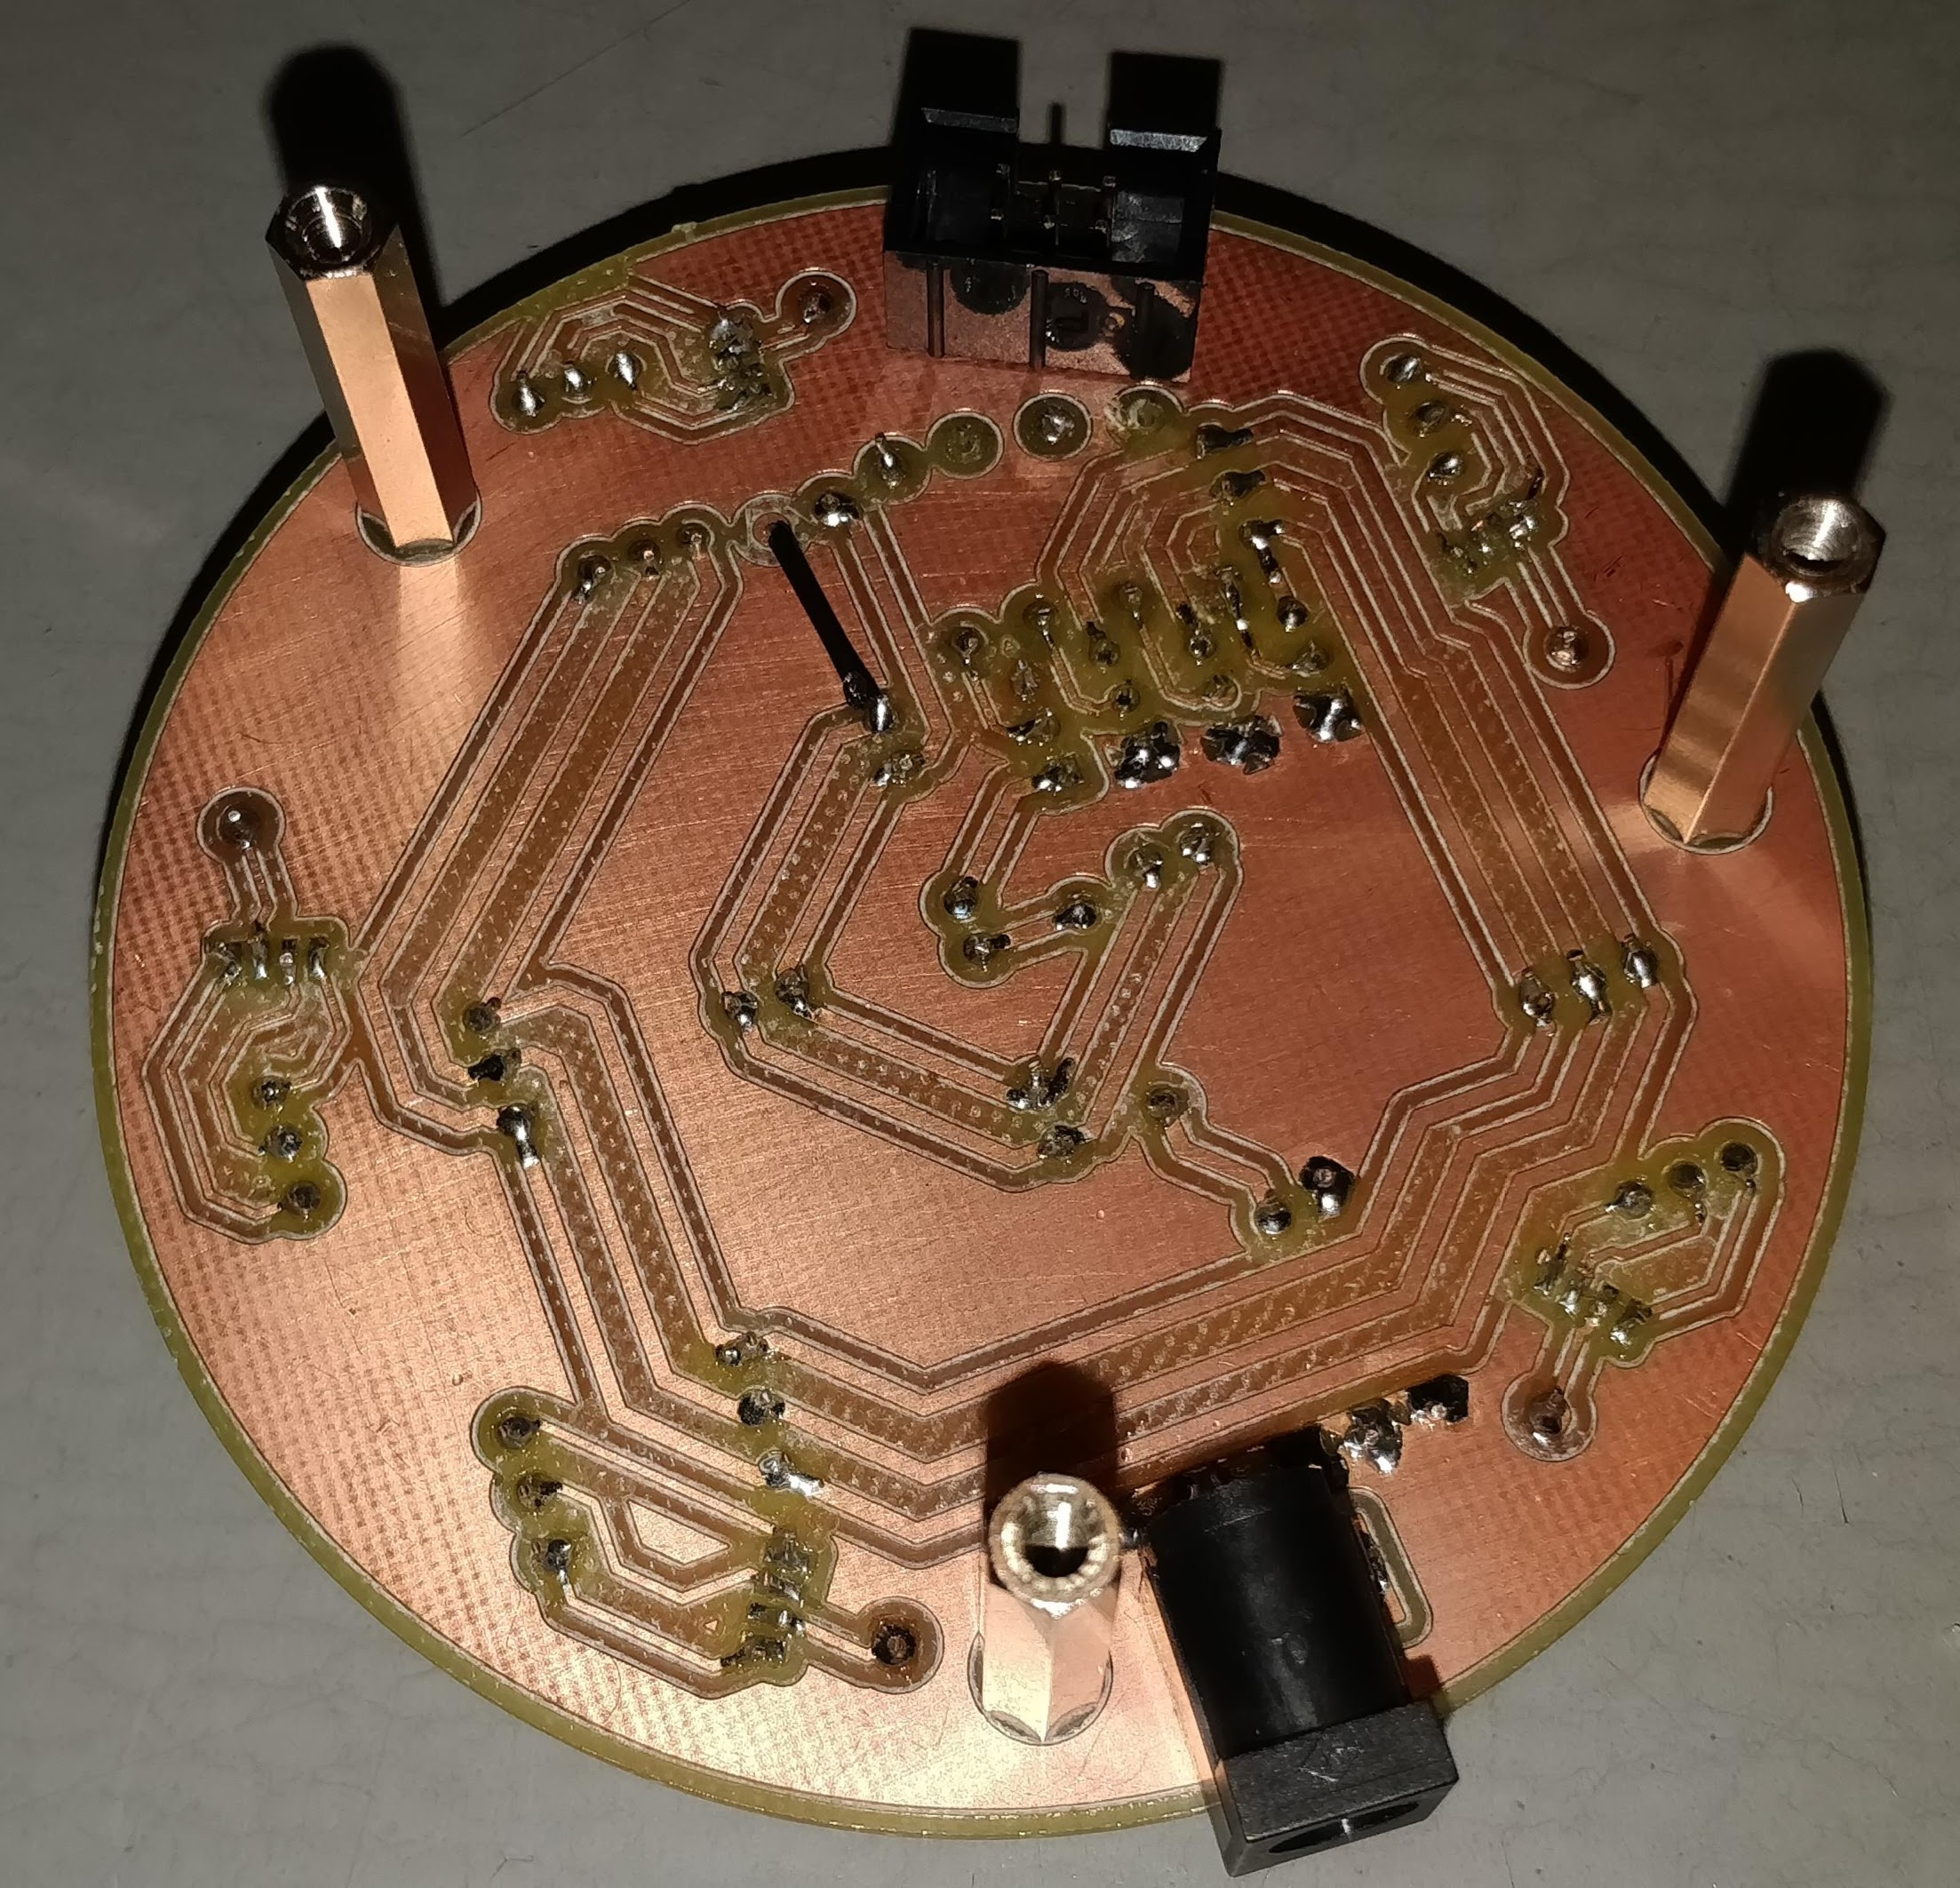
\includegraphics[width=1\linewidth]{HardwareDesign/CupHolder/graphics/bund_rev_1.jpg}
\end{subfigure}%
\begin{subfigure}{.561\textwidth}
  \centering
    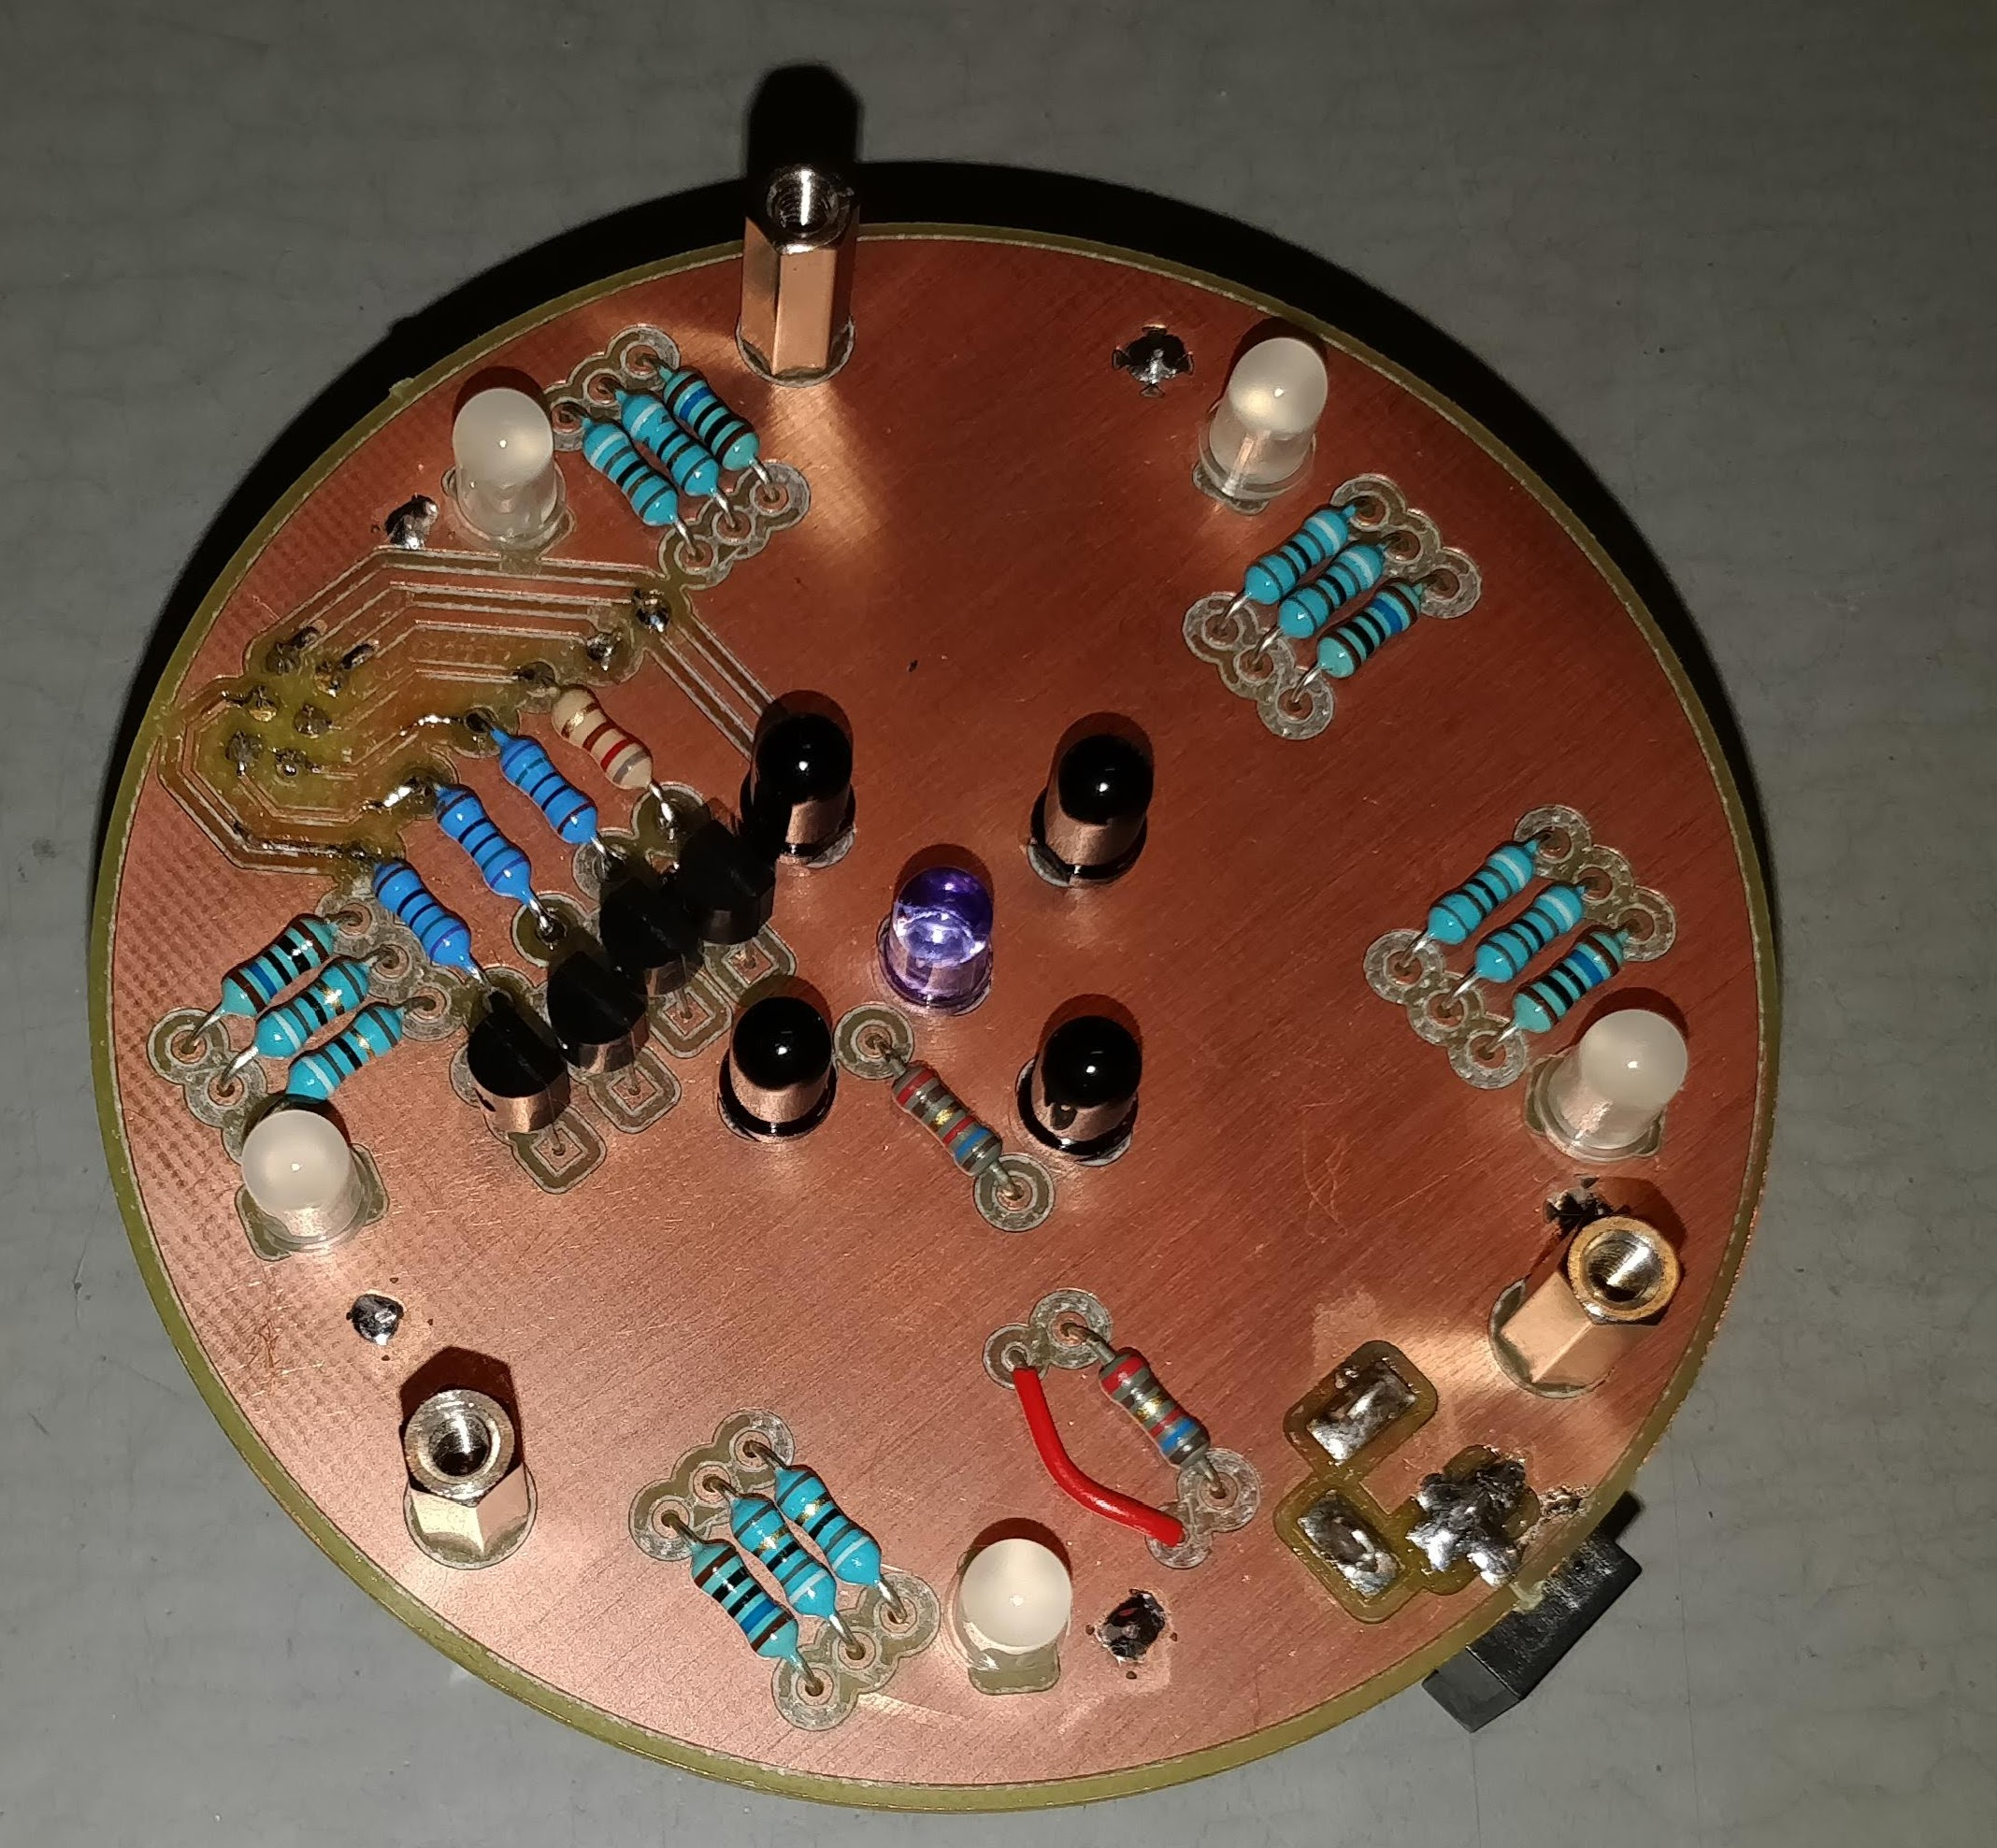
\includegraphics[width=1\linewidth]{HardwareDesign/CupHolder/graphics/top_rev_1.jpg}
\end{subfigure}
}
\caption{Den første version af Cup Holder printplade, som blev produceret af ASE, hvor der ikke er gennemplatering, soldermaske og silkscreen. På venstre figur ses bunden af printpladen. På højre side figur ses toppen af printpladen.}
\label{fig:CupHolderRev1}
\end{figure}

\begin{figure}[H]
\centering
\makebox[\textwidth][c]{%
\begin{subfigure}{.53\textwidth}
  \centering
        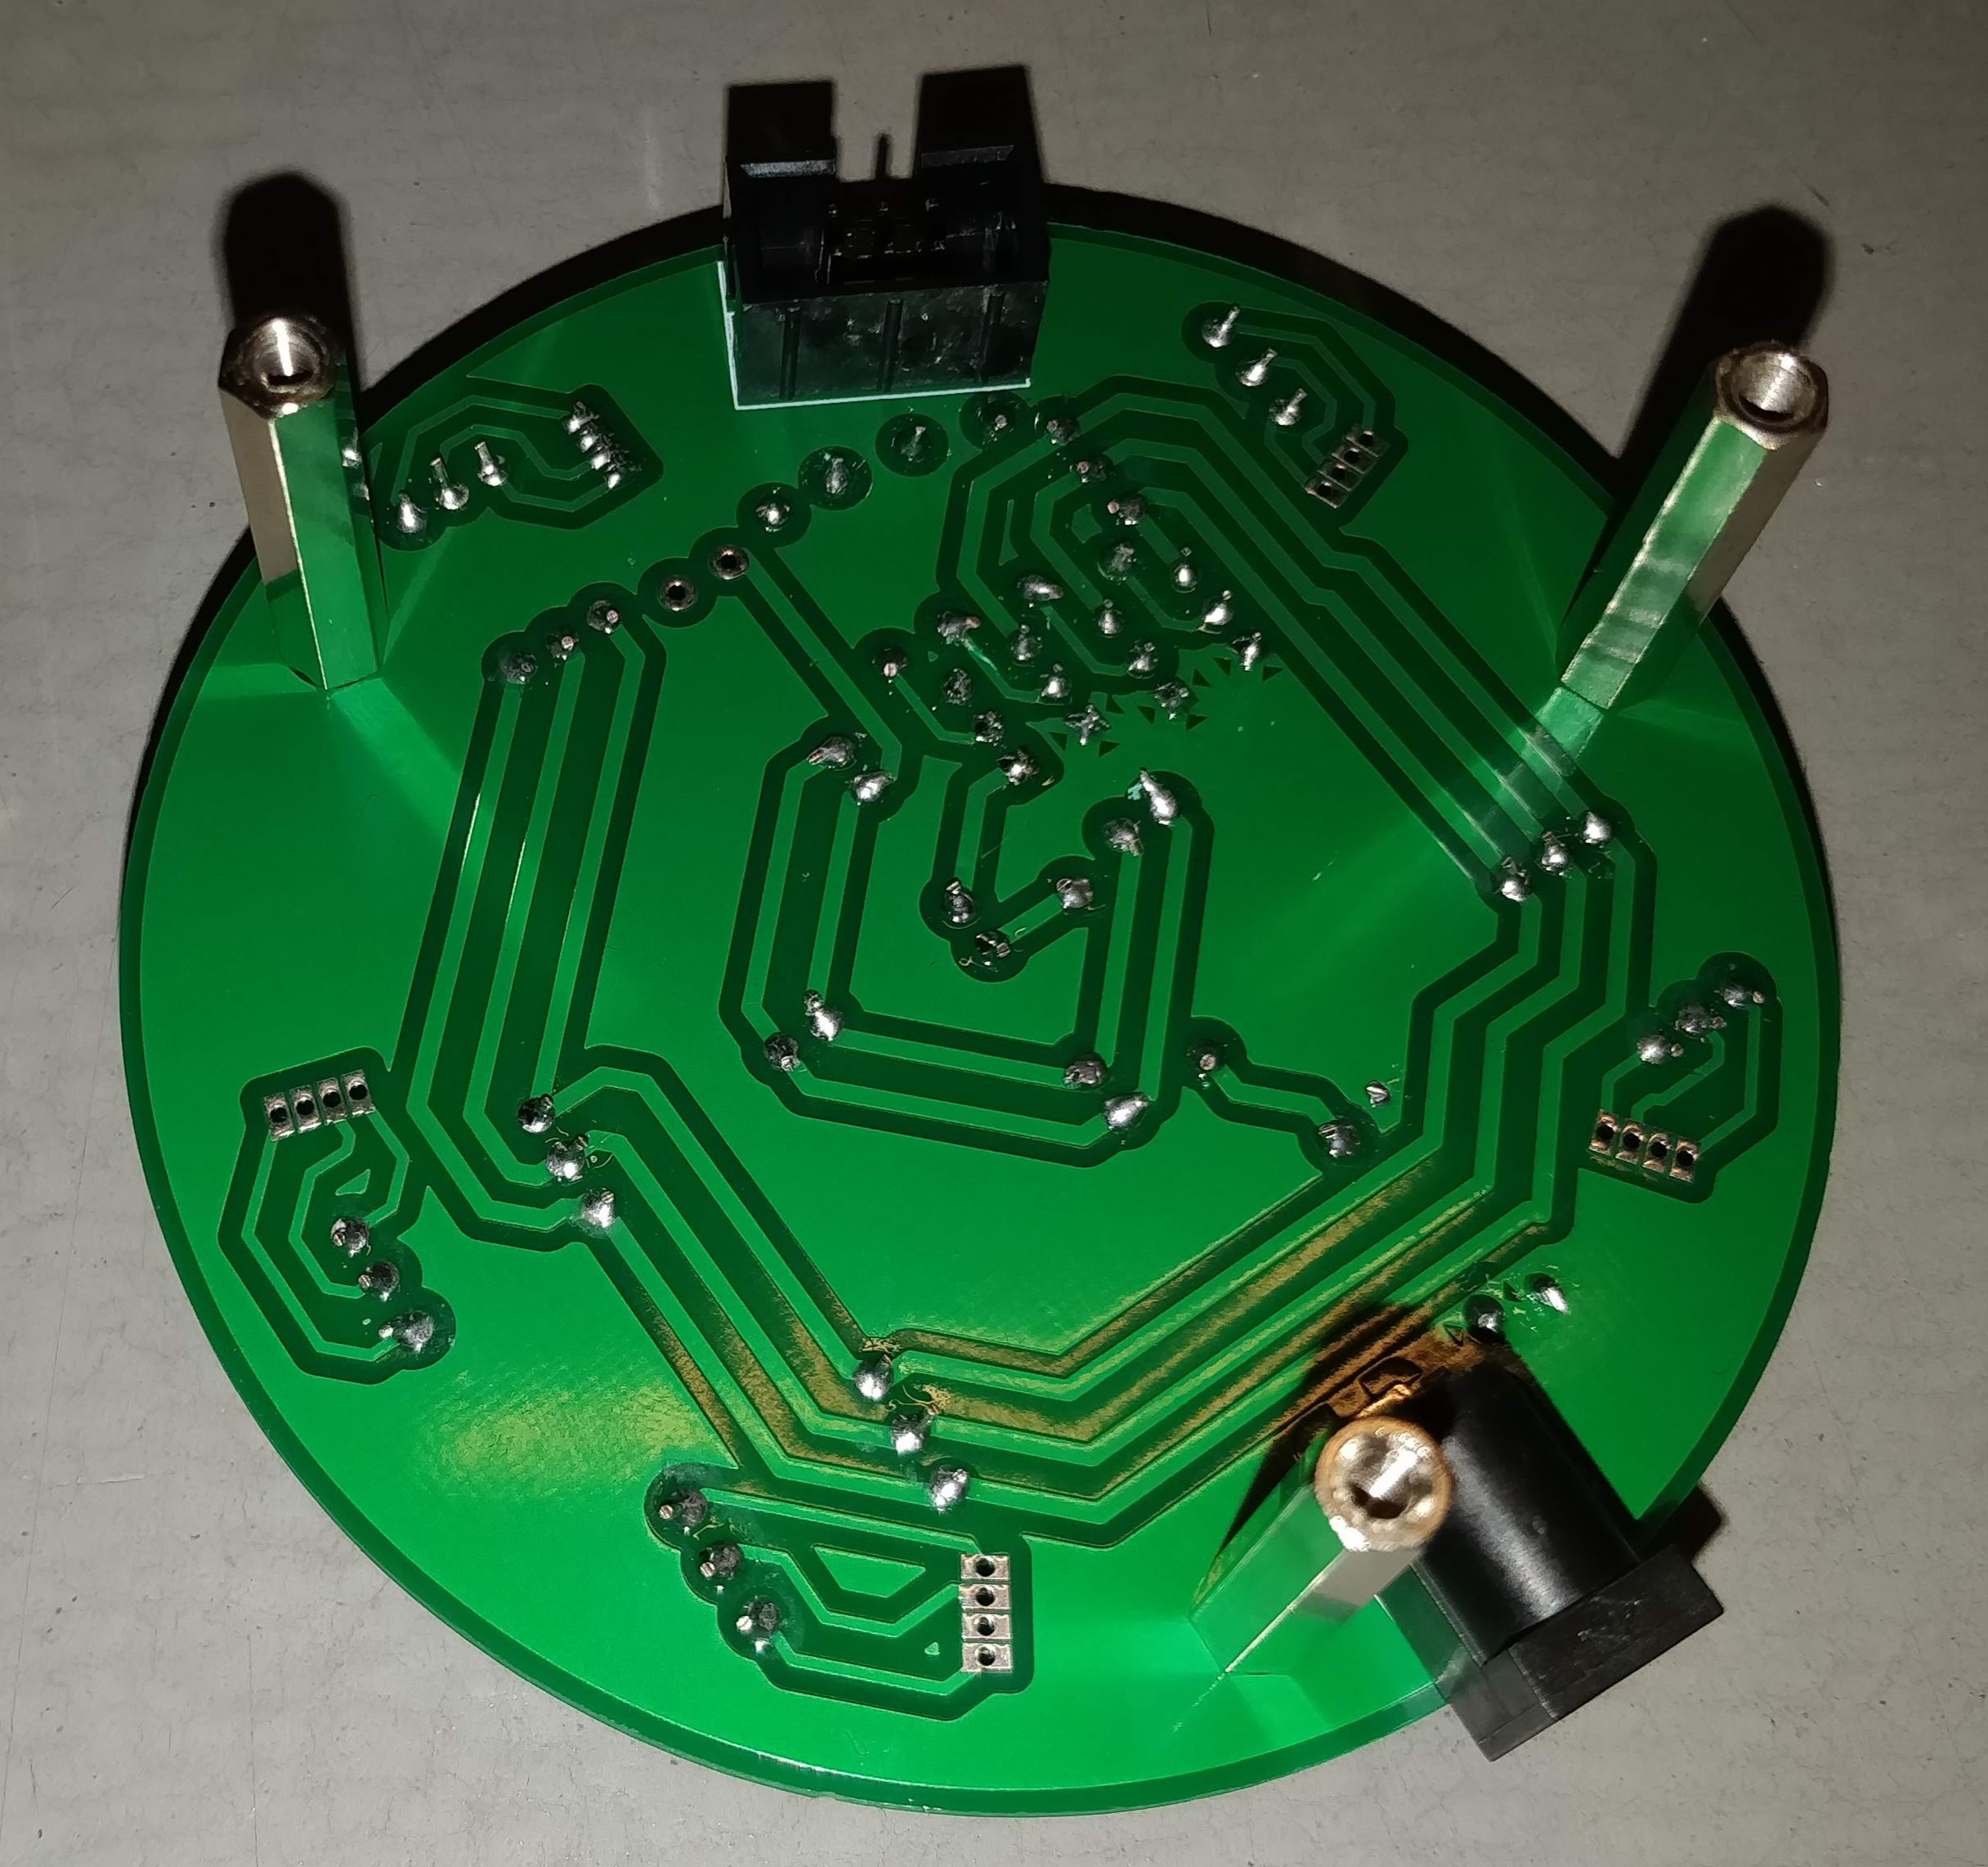
\includegraphics[width=1\linewidth]{HardwareDesign/CupHolder/graphics/bund_rev_2.jpg}
\end{subfigure}%
\begin{subfigure}{.57\textwidth}
  \centering
    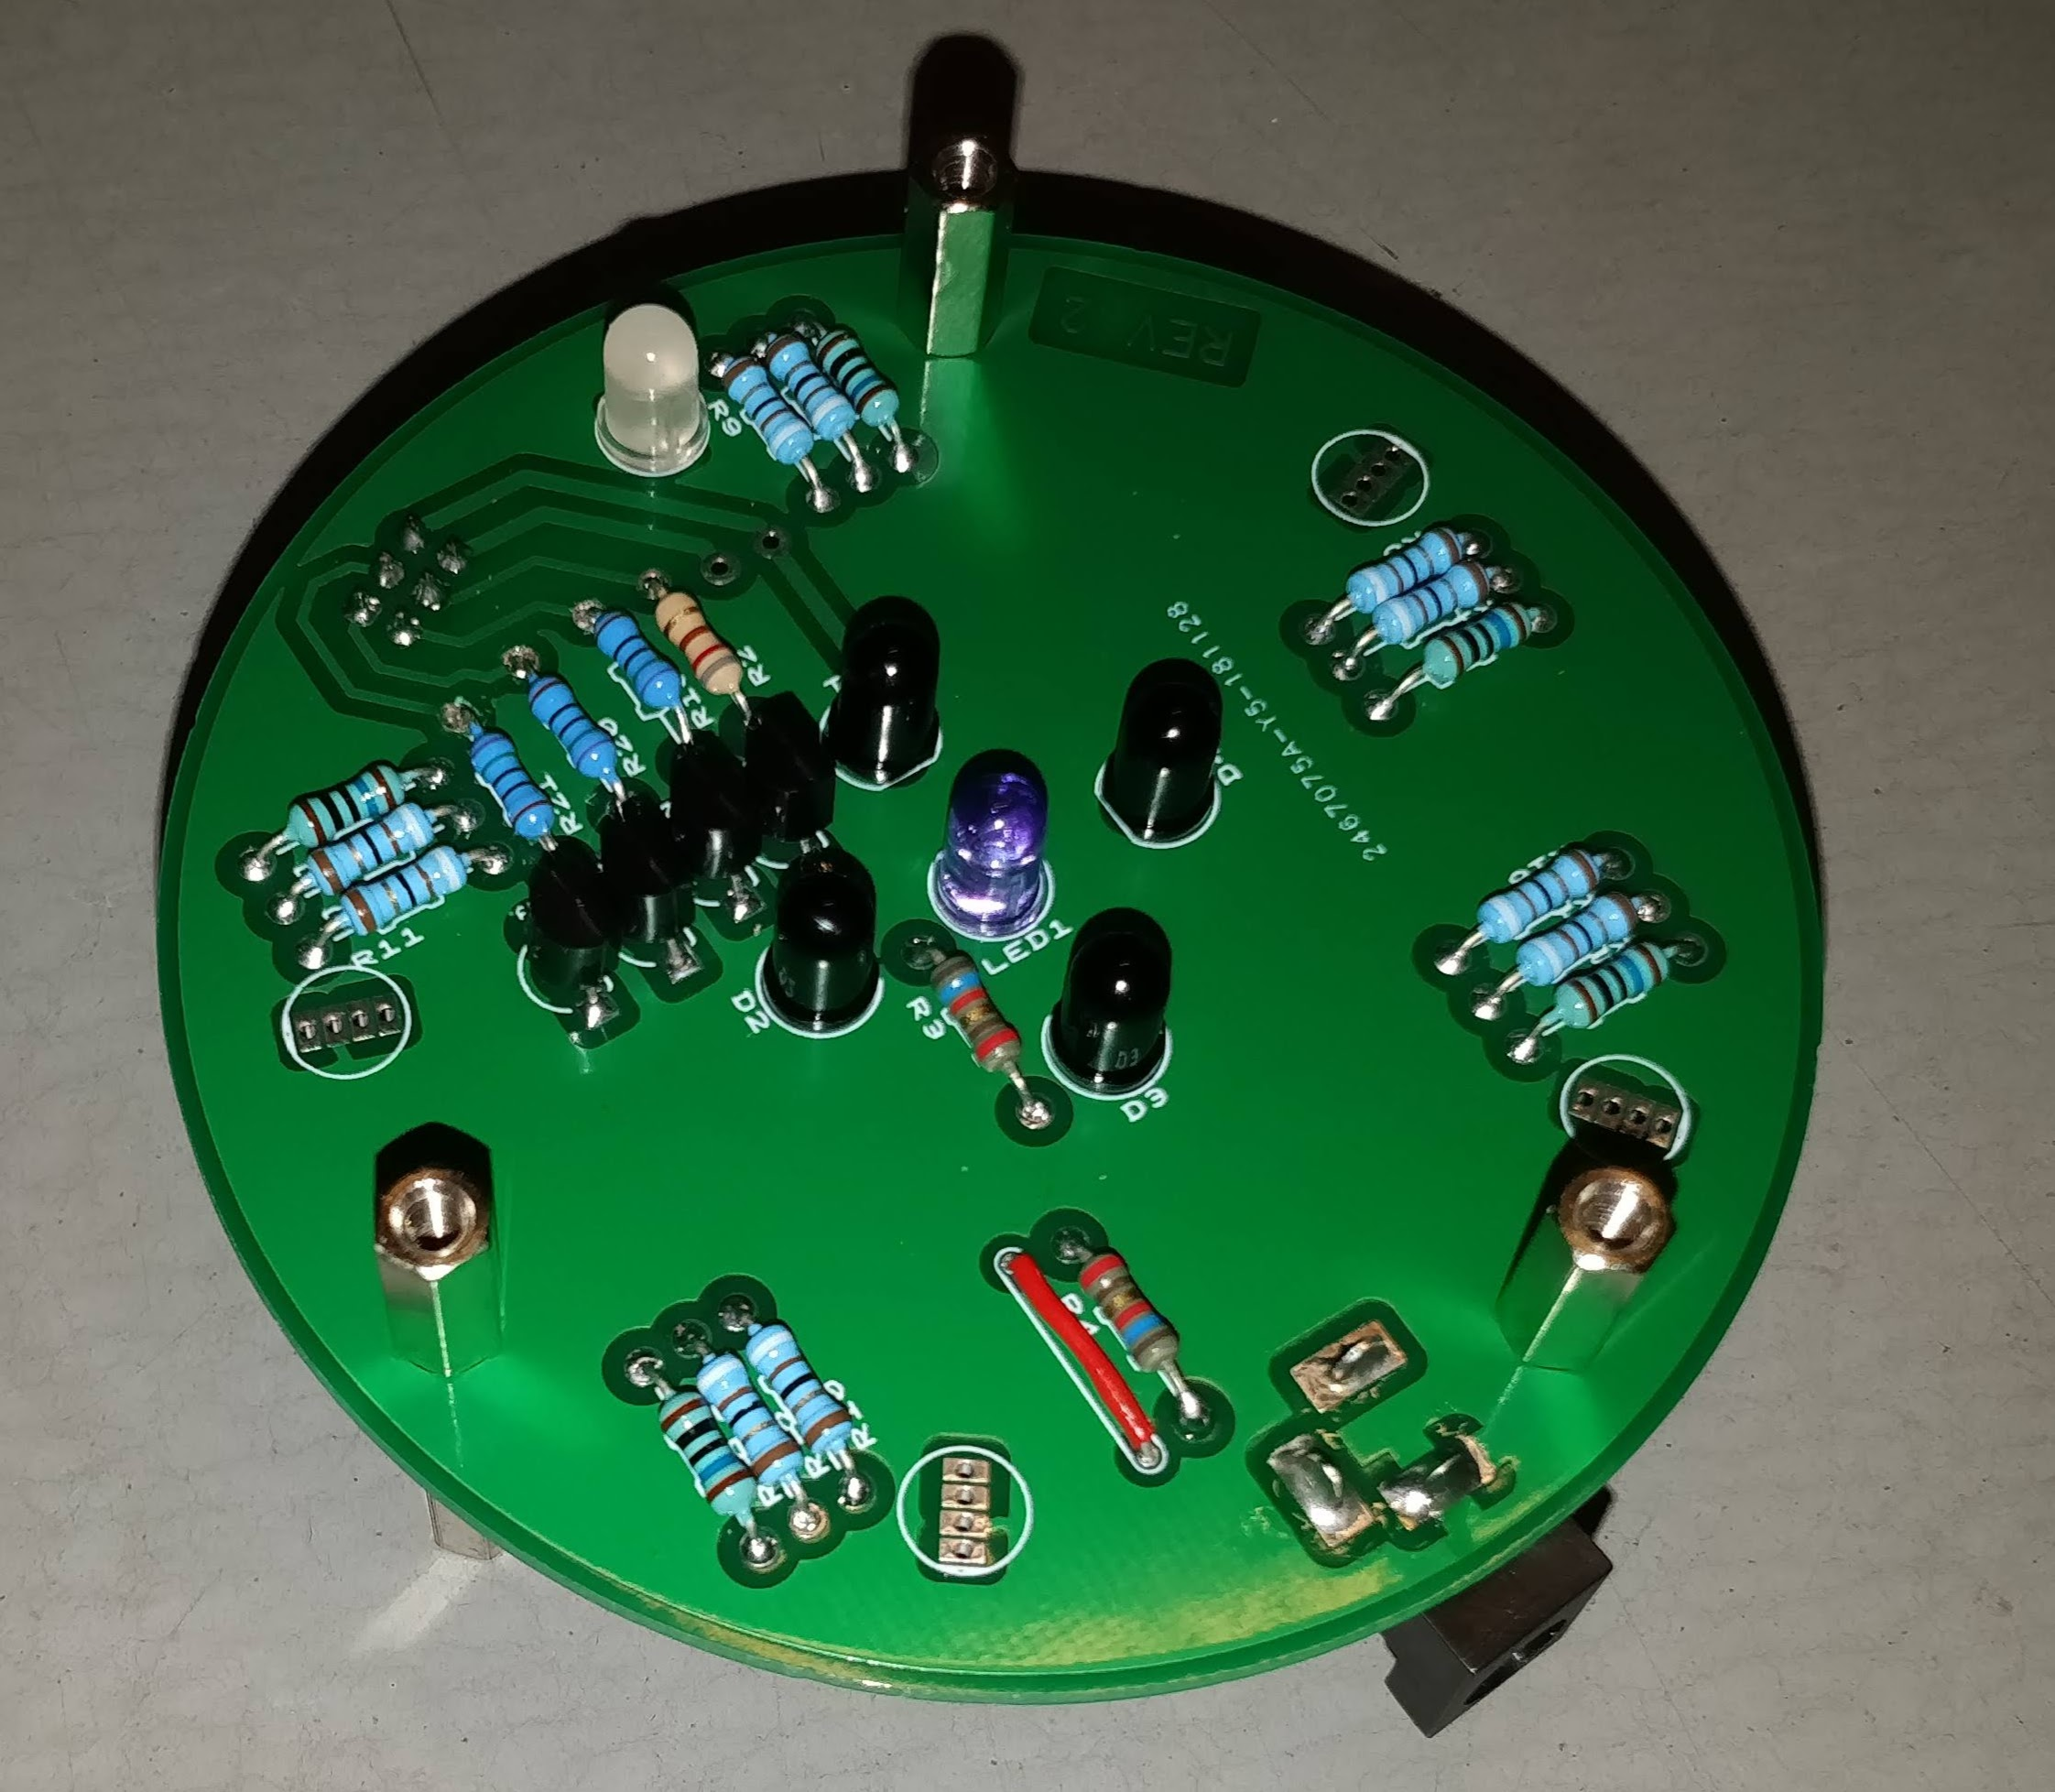
\includegraphics[width=1\linewidth]{HardwareDesign/CupHolder/graphics/top_rev_2.jpg}
\end{subfigure}
}
\caption{Den anden version af Cup Holder printplade (REV 2), som blev produceret i Kina, hvor der er gennemplatering, soldermaske og silkscreen. På venstre figur ses bunden af printpladen. På højre side figur ses toppen af printpladen.}
\label{fig:CupHolderRev2}
\end{figure}

\end{document}